\documentclass{kthreport}

\usepackage{hhline}
\usepackage[parfill]{parskip}
\usepackage{subcaption}
\usepackage{placeins}
\usepackage{todonotes}
\usepackage{graphicx,wrapfig,lipsum}

\pagestyle{plain}
\pagenumbering{arabic}

\title{Classification of ImageNet with Convolutional Neural Networks}
\subtitle{A study in techniques to improve CNN's}
\author{W. Skagerström, T. Price, N. Lindqvist}
\diarienr{Deepl-18 Project}

\begin{document}
\maketitle
\newpage
\begin{abstract}

\noindent This report is our final piece of work in the course DD2424, Deep Learning in Data Science. The overarching purpose is investigating convolutional neural networks (CNNs) while applying knowledge and techniques which we've acquired in during the course.\\

\noindent To thoroughly investigate the topic a CNN will be constructed in the most vanilla way possible. The architecture will be based on research of state of the art and previous implementation on topic. The network will be optimized iteratively by more sophisticated initialization, changing activation functions and additional additional optimization and regularization such as dropout and batch normalization. The effect of each modification will be documented and analyzed. Lastly, the results is discussed on their own and in context of other ImageNet classifiers.
\end{abstract}
\newpage

\tableofcontents
\newpage

\section{Introduction}
Image classification is one of the main branches within Computer Vision. The task can be summarized as extracting features from a picture, which takes the shape of a pixel matrix containing either 1 or 3 channels (for gray-scale or RGB, respectively). Back in 2012, Convolutional Neural Networks (CNNs) began replacing the previously manually written algorithms for feature detection, and continue to hold the title as a state of the art method for image classification. The reason for the resurgence of CNNs was partly due to the winning entry of the AlexNet in the 2012 ImageNet competition \cite{krizhevsky2012imagenet}. Convolutional Neural Networks have existed for almost 20 years, but was previously limited by the availability of data and computer hardware. However, due to the great advancement of modern computers has enabled the ability to train increasingly deep and complex types of neural networks.

In 2014, another progressive leap in the development of image classification occurred with the introduction of VGGNet and GoogleNet \cite{simonyan2014very}, \cite{szegedy2016rethinking}.  Due to the possibility of creating CNNs of varying architecture and size, a modern industry standard for evaluating the performance of a network is by benchmarking it through the ImageNet dataset \cite{russakovsky2015imagenet}.


\section{Previous work}
\label{sec:PreviousWork}
Among the many entries to the ImageNet classification challenge, deep convolution network architectures such AlexNet, VGGNet and GoogleNet have proven themselves to be highly effective and has created a renewed interest in the development and optimization of such architectures. However, these different types of network comes with some individual strengths and weaknesses.

\subsection{AlexNet}
AlexNet is the network architecture that renewed the industry interest in Convolutional Neural networks. AlexNet consists of a total of 8 layers, which are 5 convolutional layers which are stacked on each other, followed by three fully connected layers. The network features two sets of of batch normalization, which are applied following each of the first two convolution layers, and a dropout occurs after each of the last two fully connected layers. Compared to the other networks mentioned here, it performs slightly worse in terms of accuracy as seen in figure \ref{wrap-fig:graph_cnns}.

\subsection{GoogleNet}
%------------------------------------------
\begin{wrapfigure}{r}{0.5\linewidth}
  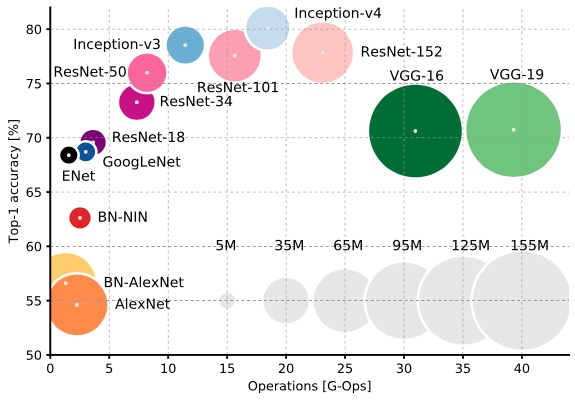
\includegraphics[width=\linewidth]{../images/graph_cnns.jpg}
  \caption[]
  {\small Comparision of performance and amount of parameters between different CNNs.}
  \label{wrap-fig:graph_cnns}
\end{wrapfigure}
%------------------------------------------
GoogleNet uses what is called a inception module, which works by calculating several different convolutions of different dimension within the same module combining them before propagating them to the next layer of the network\cite{szegedy2016rethinking}. This causes GoogleNet to be much more space efficient due to the less numerous amount of parameters, which is only further amplified by the usage of average pooling instead of fully connected layers, which further reduces the dimensionality of the total number of network parameters, see figure \ref{wrap-fig:graph_cnns}.

\subsection{ResNet}
ResNet was added to the different architectures of networks for image classification in 2015 and won the 1st place on the ILSVRC 2015 classification task. As deeper networks are more difficult to train a residual learning framework eases the training for deep networks by adding a shortcut between layers. The shortcut decreases the complexity of the networks and witch allows more layers \cite{HeZRS15}.

\subsection{VGGNet}
VGGNet was introduced in 2014 and one of its most common characteristics is the simplicity of the network, while still achieving good performance on complicated classification tasks such as the ImageNet challenge \cite{simonyan2014very}. While being simple in its design, the network is computationally demanding to train due to the heavy number of parameters.


\section{Method}
This section covers our CNN, the methods used for improving its performance, and the tools utilized for the implementation.

\subsection{Dataset}
The data used was the ImageNet Tiny dataset, which is a reduced variant of the ImageNet set. The Tiny variation consists of 200 different classes. The resolution of the images has been reduced to $64\times64\times3$ (from  $224\times224\times3$). The dataset consists of 100 000 training samples, 10000 validation samples, and 10000 test samples.
Figure \ref{fig:30_samples} visualizes a small sample of pictures included in the dataset.

\begin{figure}[htbp]
  \centering
  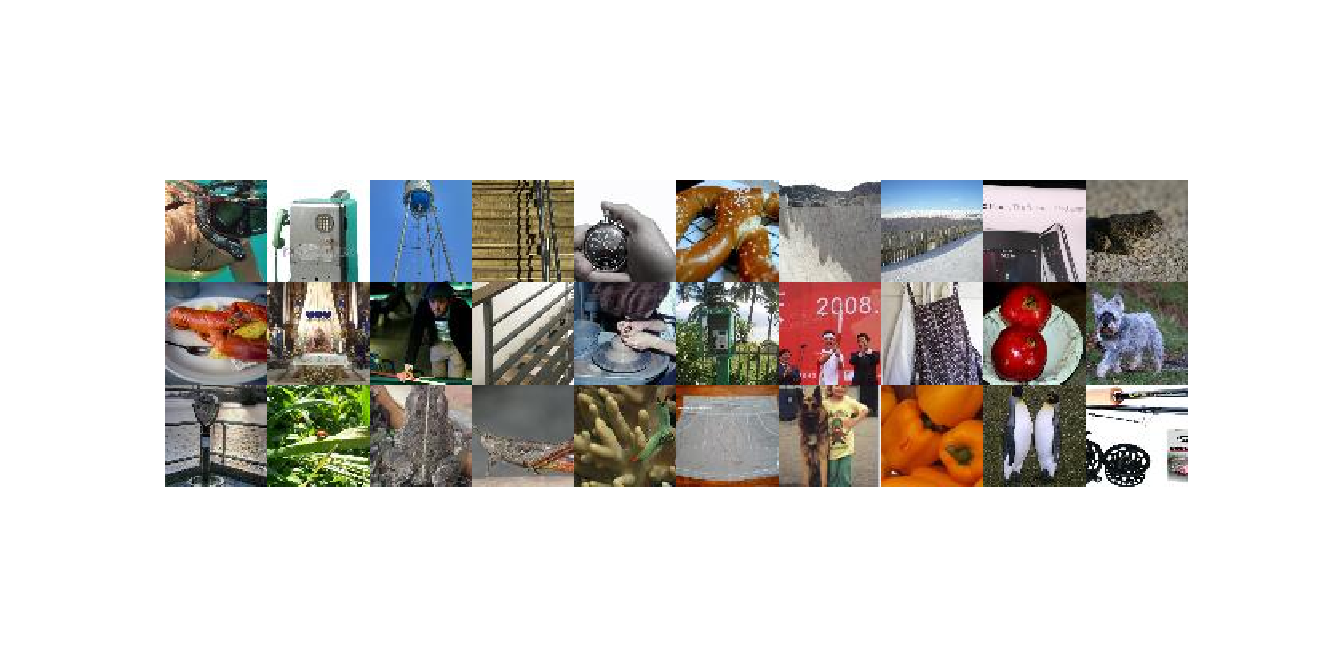
\includegraphics[width=\linewidth]{../images/samples.png}
  \caption[]
  {\small
    30 Samples from the Tiny ImageNet dataset.
  }
  \label{fig:30_samples}
\end{figure}


\subsection{Data Augmentation}
An additional feature that was later added in order to improve the accuracy of the network was data augmentation. Data augmentation was applied batch by batch for each batch used in the training process. The methods of augmentation were the following:

\begin{itemize}
  \item \textbf{Featurewise center:} Set mean of all inputs to 0.
  \item \textbf{Whitening (ZCA):} Applying whitening, may strengthen structure of objects in image by removing redundant information.
  \item \textbf{Horizontal flip:} New perspective on images naturally expands the training data. Vertical flip is available too but in many of the classes an upside-down representation has low resemblance to the image class.
  \item \textbf{Shift:} Shifting images horizontally and vertically allows images to appear in different regions of input space which allows for better generalization.
\end{itemize}

\subsection{CNN implementation}

We chose to experiment with different variations of the VGGNet architecture due to its simple implementation and the availability of hardware from the Google Cloud Computing services obtained by KTH for the DD2424 course.

\subsubsection{Implementation specifics}

The network was written and implemented in Python 3.5.2, using the Keras Framework which runs on top of Tensorflow. Numpy was used for data management and Matplotlib to create the graphs. To assist in training and evaluating the networks, we used Google Cloud services for computation power. The specifications of the hardware used was:

\begin{itemize}
  \item 1 x NVIDIA Tesla K80
  \item An unspecified dual core CPU (Unknown CPU Platform on the Google Cloud Platform).
  \item 16 GB RAM memory
  \item 40 GB Disk space.
\end{itemize}

\subsection{Normalization}
Normalization of the input data occurs as two different methods: At first, some models are trained with data where the color channels are divided by the maximum output of the RGB color palettes (255), resulting in the the colors being represented as numbers in ${\rm I\!R} \in [0,1]$.
This was later changed to using Batch Normalization instead for the later training iterations.

\subsubsection{Evaluating architectures}

The basis of the CNN architecture is inspired by \cite{NIPS2012_4824}, it is summarized in figure \ref{fig:architecture}. However, it was implemented on the full ImageNet dataset. Inspired by architectures mentioned in Previous work \ref{sec:PreviousWork}, we decided to test three configurations, summarized in \ref{table:3_configurations}.

\medskip
\begin{table}[htbp]
\begin{center}
\begin{tabular}{|c|c|c|}

  \hline
  \multicolumn{3}{|c|}{ConvNet Configuration} \\
  \hline

  A & B & C
  \\\hline

  X weight layers & Y weight layers & Z weight layers
  \\\hhline{|=|=|=|}

  \multicolumn{3}{|c|}{input ($64\times64\;RGB\;image$)}
  \\\hline

  conv3-64 & conv3-64 & conv3-64
  \\\hline

  \end{tabular}
\caption[]
{\small
  Configuration of the three different CNNs tested initially. They are inspired from (A) reference, (B) reference and (C) reference.
}
\label{table:3_configurations}
\end{center}
\end{table}


% We should not use this anymore(?)
% \begin{figure}[htbp]
  \centering
  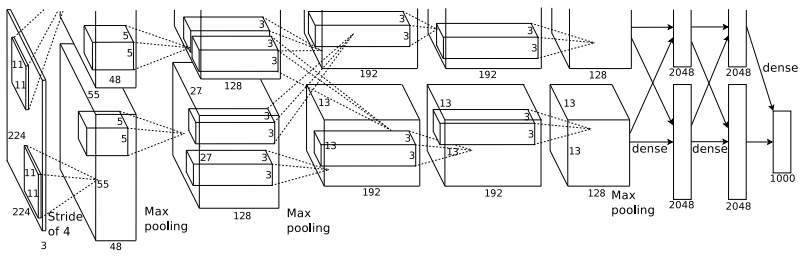
\includegraphics[width=\linewidth]{../images/architecture.jpg}
  \caption[]
  {\small
    Overview of network architecture presented by \cite{NIPS2012_4824}.
  }
  \label{fig:architecture}
\end{figure}


Tests was run with \textbf{insert how tests were run} iterations. Training was done on the entire Tiny Imagenet dataset, containing 100 000 images and their respective labels. The composition of the dataset is 200 classes with 500 images each. The training data is shuffled before the training process begins. For evaluation, the entire validation dataset was used, containing 10000 images. The results of each architecture is presented in section...

\subsubsection{Initialization matters}

Details about the different parts of the network.\\
Weight initialization.\\
Optimizer.\\
Learning rate.\\
Loss function.\\




\subsubsection{Training and evaluation}
The network was trained on the entire Tiny ImageNet dataset, consisting of the 100 000 pictures, for \textbf{NUMBER OF EPOCHS}. Some of the later iterations of training also included data augmentation methods listed in \textbf{WHERE DATA AUGMENTATION SECTION IS}.

\section{Results}

\subsection{Declaring war on overfitting}

Running over all 4 models presented in table \ref{table:3_configurations} the training and validation loss proved immense after around 10 epochs. See figure \ref{fig:4_losses}. We then realized that most of the architectures lacked any form of regularization, rendering our results very much expected.

\begin{figure*}
        \centering
        \begin{subfigure}[b]{0.475\textwidth}
            \centering
            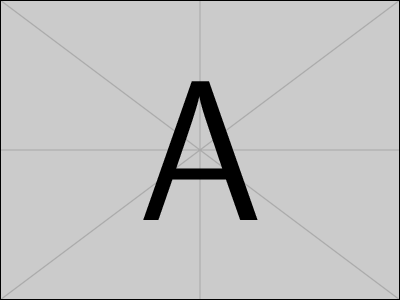
\includegraphics[width=\textwidth]{../images/example-image-a.png}
            \caption[Network2]%
            {{\small Network 1}}
        \end{subfigure}
        \hfill
        \begin{subfigure}[b]{0.475\textwidth}
            \centering
            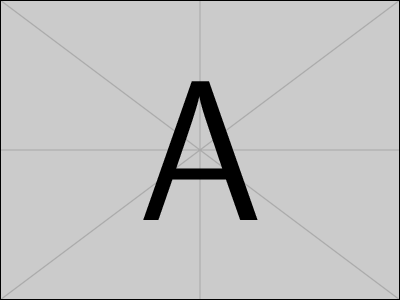
\includegraphics[width=\textwidth]{../images/example-image-a.png}
            \caption[]%
            {{\small Network 2}}
        \end{subfigure}
        \vskip\baselineskip
        \begin{subfigure}[b]{0.475\textwidth}
            \centering
            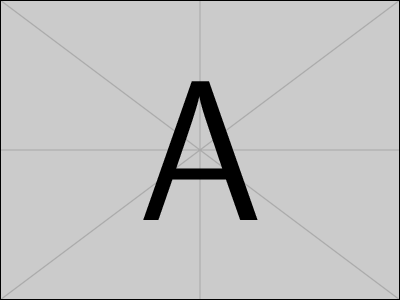
\includegraphics[width=\textwidth]{../images/example-image-a.png}
            \caption[]%
            {{\small Network 3}}
        \end{subfigure}
        \quad
        \begin{subfigure}[b]{0.475\textwidth}
            \centering
            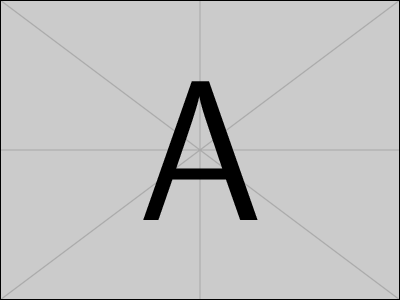
\includegraphics[width=\textwidth]{../images/example-image-a.png}
            \caption[]%
            {{\small Network 4}}
        \end{subfigure}
        \caption[ The average and standard deviation of critical parameters ]
        {\small Caption}
        \label{fig:4_losses}
    \end{figure*}


To combat the overfitting we begun tinkering with what regularization techniques are known to us, these were:

\begin{itemize}
  \item Subtracting mean of all images
  \item L2 regularization
  \item Dropout in dense layers
  \item Decay rate
\end{itemize}

Manually tuning these parameters we found some improvements, such as those in figure \ref{fig:loss_improved_1}. And continuing in the same manner gave the loss plot of figure REF.

\begin{figure}[htbp]
  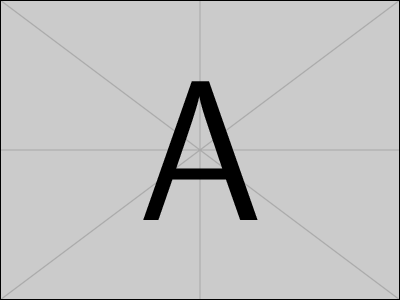
\includegraphics[width=\linewidth]{../images/example-image-a.png}
  \caption{Caption}
  \label{fig:loss_improved_1}
\end{figure}


\subsection{Final results}

The final results found was achieved with a model of with \textbf{SPECS}.

The top-1 accuracy was \textbf{X} and top-5 accuracy \textbf{Y}. This indicates \textbf{Z}.

% Graphs/Tables of trainloss, valloss, accuracies etc.
% 

\begin{figure}[!h]
\begin{subfigure}{.5\textwidth}
  \centering
  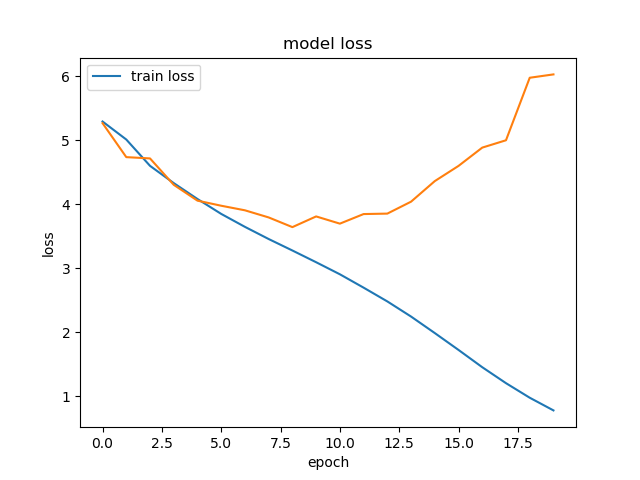
\includegraphics[width=1.1\linewidth]{../../src/loss_plots/sgd.png}
  \caption{Accuracy}
  \label{fig:sfig1}
\end{subfigure}%
\begin{subfigure}{.5\textwidth}
  \centering
  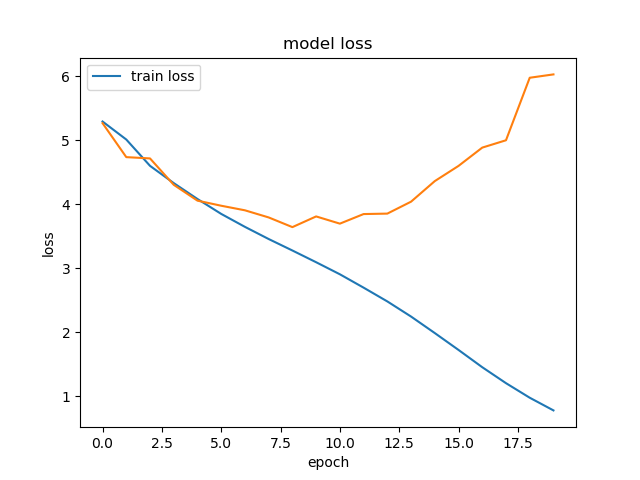
\includegraphics[width=1.1\linewidth]{../../src/loss_plots/sgd.png}
  \caption{Loss}
  \label{fig:sfig2}
\end{subfigure}
\caption{SGD something something}
\label{fig:fig}
\end{figure}
\FloatBarrier


\section{Discussion}

\subsection{Evaluation of method}
Thoughts about the method.

If we where to recreate the experiment we would use a different base architecture for the network.
As seen in figure \ref{wrap-fig:graph_cnns} it is clear that using an VGG structure is not optimal in regard to accuracy, operations and amount of parameters.
A residual network structure seems to be the network with the highest potential today with regard to accuracy and operation.
We would probably start with a basic ResNet structure instead of the VGG-net.
The reason for using a VGG- net was foremost its easy interpretation and simple implementation. However, the struggle to get an high accuracy due to slow training rate most likely slowed down the process more then the time required to implement and interpret the ResNet structure.

Ignoring all gray-scale images in training could have an slight impact on our test accuracy. If we were to recreate the method we would try to figure out an optimal way of handling both grayscale images and RGB images in the same method. One approach would be to reduce all images with 3 channels to grayscale images and create a model optimal for only 1 channel images. Another approach would be to use a assemble methodology with one network adapted for grayscale images and one for RGB images.

\subsection{Evaluation of results}

Thoughts about the result.

As mentioned in the previous section the test accuracy would perhaps have been slightly higher if we would have regarded the fact that some images are in gray-scale. Around 2\% of the test images and validation images are gray-scale and we assume that the percentage of gray-scale images is the same in the test data. This implies an 2\% loss in accuracy on the test data.

\subsection{ImageNet state of the art}

Comparing ours to other state of the art networks.

In Techniques for Image Classification on Tiny-ImageNet by Zach Barnes, Frank Cipollone and Tyler Romero of Stanford University, Stanford, CA they showed that using a ResNet18 with data augmentation, dropout and Snapshot Ensembleling they could receive an accuracy of top-5 validation of 81,4 \%, top-1 validation of 60,2 \% and top-1 test of 53,6 \%.


DenResNet: Ensembling Dense Networks and Residual Networks by Victor Cheung of Stanford University Computer Science Department achieve an accuracy of approximately 0.65 top-1 error rate on the validation set and an error on the test set of 25.6. As of June 12th, 2017 their result was first on the leaderboard for TinyImagenet. They used a  ensemble of three models: ResNet101, ResNet152 and DenseNet121. They apply normalization, marginalization and MAP inference in the ensemble architecture.

\section{Conclusion}
Final thoughts, future research, improvements etc.



\bibliography{references}{}
\bibliographystyle{plain}

\end{document}
